	\documentclass[10pt,oneside]{CBFT_book}
	% Algunos paquetes
	\usepackage{amssymb}
	\usepackage{amsmath}
	\usepackage{graphicx}
	\usepackage{bm}
% 	\usepackage{libertine}
	\usepackage[bold-style=TeX]{unicode-math}
	\usepackage{lipsum}

	\usepackage{natbib}
	\setcitestyle{square}

	\usepackage{polyglossia}
	\setdefaultlanguage{spanish}


	\usepackage{CBFT.estilo} % Cargo la hoja de estilo

	% Tipografías
	% \setromanfont[Mapping=tex-text]{Linux Libertine O}
	% \setsansfont[Mapping=tex-text]{DejaVu Sans}
	% \setmonofont[Mapping=tex-text]{DejaVu Sans Mono}

	%===================================================================
	%	DOCUMENTO PROPIAMENTE DICHO
	%===================================================================

\begin{document}

% =================================================================================================
\chapter{Teorema de Green}
% =================================================================================================

% =================================================================================================
\section{Imágenes y método de Green}
% =================================================================================================

El método de las imágenes es un procedimiento gráfico de encontrar problemas equivalentes simulando
con cargas extras (cargas imagen) las condiciones de contorno.

\begin{figure}[htb]
	\begin{center}
	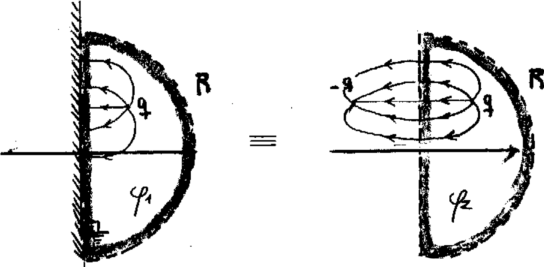
\includegraphics[width=0.6\textwidth]{images/fig_ft1_imagegreen1.pdf}	 
	\end{center}
	\caption{}
\end{figure} 

Los problemas que ilustra la figura satisfacen iguales condiciones de contorno en el recinto punteado,
entonces sus soluciones internas son la misma: $\phi_1 = \phi_2$ por unicidad.

\subsection{El Método de Green}

El concepto tras el método de Green es evaluar el $\phi$ de una carga puntual ante cierta configuración
de contornos conductores. Es una excitación elemental.

Restando entre sí
\[
	\Nabla\cdot(\phi\Nabla\psi) = \phi\lapm{\psi} + \Nabla\phi\cdot\Nabla\psi
\]
y
\[
	\Nabla\cdot(\psi\Nabla\phi) = \psi\lapm{\phi} + \Nabla\psi\cdot\Nabla\phi
\]
e integrando ambos miembros y utilizando el teorema de la divergencia, se llega a
\[
	\int_V \left[ \phi\lapm{\psi} - \psi\lapm{\phi}\right] dV =
	\int_S \left[ \phi\Nabla\psi - \psi\Nabla\phi \right] dS,
\]
que es la segunda identidad de Green.

Consideremos lo que llamaremos caso A, según vemos en figura, caracterizado según
\[
	\rho_{int} \qquad \vb{x}'\in R, \vb{x}\in R
\]
\begin{figure}[htb]
	\begin{center}
	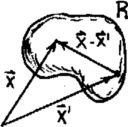
\includegraphics[width=0.2\textwidth]{images/fig_ft1_imagegreen2.pdf}	 
	\end{center}
	\caption{}
\end{figure} 
\[
	\psi = \frac{1}{|\vb{x}-\vb{x}'|} \qquad \lapm{\psi} = -4\pi \delta(\vb{x}-\vb{x}')
\]
\[
	-\phi(\vb{x})4\pi + \int_V 4\pi \frac{\rho(\vb{x}')}{|\vb{x}-\vb{x}'|} \; dV' =
	\int_S \left( \phi\dpar{\psi}{n}-\frac{1}{|\vb{x}-\vb{x}'|}\dpar{\phi}{n}\right)\; dS 
\]
donde estamos usando la abreviatura $\Nabla\phi\cdot\vb{n}=\partial\phi/\partial n$ que es la
derivada normal en la superficie. Despejando
\[
	\phi(\vb{x}) = \int_V \frac{\rho(\vb{x}')}{|\vb{x}-\vb{x}'|} \; dV' +
	\frac{1}{4\pi} \int_S \left( \frac{1}{|\vb{x}-\vb{x}'|}\dpar{\phi}{n} -\phi\frac{\partial}{\partial 
n} \left[\frac{1}{|\vb{x}-\vb{x}'|} \right] \right)\; dS ,
\]
donde la primer integral es debido a las cargas internas y la segunda al efecto de las cargas
fuera del reciento $R$.

Recordemos que las condiciones tipo Dirichlet corresponden a $\phi|_S$ y las tipo Neumann a
$\partial\phi/\partial \hat{n}|_S$.

El caso B, según figura, corresponde a
\[
	\rho_{int} \qquad \vb{x}'\notin R, \vb{x}\in R
\]
y 
\[
	\int_V \frac{\rho(\vb{x}')}{|\vb{x}-\vb{x}'|} \; dV' = 
	\frac{1}{4\pi} \int_S \left( \phi\frac{\partial}{\partial n} \left[\frac{1}{|\vb{x}-\vb{x}'|} \right]
	- \frac{1}{|\vb{x}-\vb{x}'|}\dpar{\phi}{n}  \right)\; dS ,
\]
la integral de superficie proviene de las cargas fuera de $R$ que producen campo en el interior
$R$.

\begin{figure}[htb]
	\begin{center}
	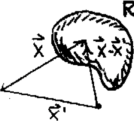
\includegraphics[width=0.2\textwidth]{images/fig_ft1_imagegreen3.pdf}	 
	\end{center}
	\caption{}
\end{figure} 

Hemos tomado $\psi=1/|\vb{x}-\vb{x}'|$ que verifica [1]; interpretándose $\psi$ como el potencial
de una carga puntual unitaria.

\[
	\lapm{\frac{1}{|\vb{x}-\vb{x}'|}} = - 4\pi \delta( |\vb{x}-\vb{x}'| )
\]
podemos tomar
\[
	G \equiv \frac{1}{|\vb{x}-\vb{x}'|} + f( \vb{x}, \vb{x}')
\]
donde $G$ es la función de Green.

\[
	\lapm{G} = -4\pi  \delta( \vb{x}, \vb{x}' ) + \lapm{f}
\]
donde $F$ satisface Laplace (si el reciento no incluye a $\vb{x}'$).
Con $\lapm{f( \vb{x}, \vb{x}' )}$.

Entonces $f( \vb{x}, \vb{x}' )$ representan la o las imágenes necesarias para que
$G$ cumpla el contorno necesario $G_D|_S=0$.


% =================================================================================================
\section{Funciones de Green}
% =================================================================================================

\be
	\phi(\vb{x}) = \int_{V'} G(\vb{x},\vb{x}') \rho(\vb{x}')  \; dV' +
	\frac{1}{4\pi} \int_{S'} \left( G(\vb{x},\vb{x}')\dpar{\phi}{n} -\phi\frac{\partial}{\partial 
	n} G(\vb{x},\vb{x}') \right)\; dS' ,
	\label{green1}
\ee
Pero para poder utilizar \eqref{green1} necesito tener un solo tipo de condiciones de contorno,
de manera que según sean
\[
	\textrm{Dirichlet} \quad 	\begin{cases}
				G_D : \lapm{G_D} = -4\pi \delta(\vb{x},\vb{x}') \\
				G_D |_{contorno de R} = 0  \\
				\phi|_S \\
				\phi(\vb{x}) = \displaystyle \int_{V'} G_D \rho \; dV' - \frac{1}{4\pi}
				\int_{S} \phi|_S\frac{\partial}{\partial n} G_D \; dS'
			\end{cases}
\]
donde la condición de contorno de $G$ equivale, en el contexto físico del electromagnetismo, a
reemplazar el contorno por un conductor metálico puesto a tierra.
Entonces $G$ es el potencial de la configuración de conductores con el contorno puesto a tierra
frente a una carga puntual con magnitud unitaria.

La función de Green da la geometría del problema.

\[
	\dpar{\phi_1}{n}|_S - \dpar{\phi_2}{n}|_S = -4\pi\sigma \qquad \qquad \phi_2|_S = \phi_1|_S
\]

\[
	\textrm{Neumann} \quad 	\begin{cases}
				G_N : \lapm{G_N} = -4\pi \delta(\vb{x},\vb{x}') \\
				\Nabla G_N \cdot \hat{n}|_S = -\frac{4\pi}{S}  \\
				\left.\dpar{\phi}{n}\right|_S \\
				\phi(\vb{x}) = \displaystyle <\phi>|_S + \int_{V'} G_N \rho \; dV' + 
				\frac{1}{4\pi} \int_{S} G_N|_S \dpar{G_N}{n} \; dS
			\end{cases}
\]

\subsection{Green para el problema externo de una esfera}

En este problema las condiciones adecuadas son las de Dirichlet, ver Figura
\begin{figure}[htb]
	\begin{center}
	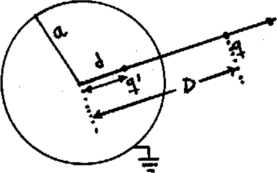
\includegraphics[width=0.4\textwidth]{images/fig_ft1_green1.pdf}	 
	\end{center}
	\caption{}
\end{figure} 
y podemos escribir la función de Green como 
\[
	G = \frac{1}{|\vb{r} - D\hat{r}'|} - \frac{a/D}{|\vb{r} - a^2/D\hat{r}'|} \qquad G|_{r=a}
\]
sujeta a que 
\[
	q' = -q a/D \qquad d = a^2/D
\]
\begin{figure}[htb]
	\begin{center}
	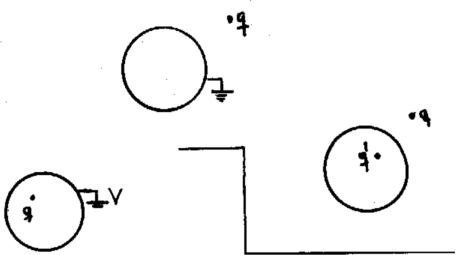
\includegraphics[width=0.6\textwidth]{images/fig_ft1_green2.pdf}	 
	\end{center}
	\caption{$G_D$ es el potencial de la configuración (a) y se evalúa teniendo en cuenta la
	otra (b) que se resuelve casualmente por imágenes. La (c) se resuelve alterando las condiciones.}
\end{figure} 

El caso (c) de la Figura se resuelve con 
\[
	-\frac{V}{4\pi} \int_S \dpar{G}{n} dS = -\frac{V}{4\pi} \int_S \Nabla G\cdot d\vb{S} =
	-\frac{V}{4\pi} \int_V \lapm{G} \: dV	
\]
\[
	= -\frac{V}{4\pi} (-4\pi)\int_V \delta(\vb{x}-\vb{x}') \: dV	= V 
\]

\section{Algunos campos}

En distribuciones infinitas de carga la integral de Poisson diverge pero ello se debe a que en
realidad no existen distribuciones infinitas de carga.
\begin{figure}[thb]
	\begin{center}
	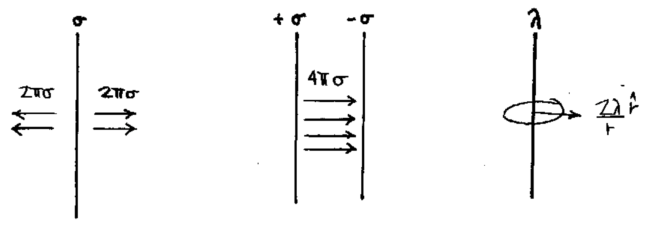
\includegraphics[width=0.8\textwidth]{images/fig_ft1_campohilos.pdf}	 
	\end{center}
	\caption{}
\end{figure} 

\section{Notas método de Green}

Función de Green libre (sin contornos) lleva directo a la integral de Poisson
\[
	G(\vb{x}, \vb{x}') = \frac{1}{|\vb{x} - \vb{x}'|}
\]
entonces 
\[
	\phi(\vb{x}) = \int_V \rho \:G \:dV = \int_{V'} \frac{ \rho(\vb{x}) }{|\vb{x}-\vb{x}'|} dV'
\]
\[
	\nabla^2 \left( \frac{1}{|\vb{x} - \vb{x}'|} \right) = 4\pi \delta(\vb{x}-\vb{x}')
\]
\[
	G(\vb{x}, \vb{x}') =  \frac{1}{|\vb{x} - \vb{x}'|} + f(\vb{x}, \vb{x}') \qquad 
	\textrm{con} \quad \lapm{f}(\vb{x}, \vb{x}') = 0 \quad \textrm{si} \quad \vb{x}\neq\vb{x}'
\]

Para condiciones de Neumann se toma:
\[
	\Nabla G_N|_S = -\frac{4\pi}{S} = \left. \dpar{G}{n} \right|_S
\]
la integral 
\[
	- \frac{1}{4\pi} \int_S \phi|_S \left.\dpar{G}{n}\right|_S  dS
\]
no se puede anular con 
\[
	\left.\dpar{G}{n}\right|_S = 0
\]
salvo que el volumen de integración no contenga a $\vb{x}=\vb{x}'$ en cuyo caso:
se excluye $\vb{x}=\vb{x}'$ de la integración.
\[
	- \frac{1}{4\pi} \int_S \phi|_S \left.\dpar{G}{n}\right|_S  dS =
	\frac{1}{S} \int_S \phi|_S dS = <\phi>|_S
\]
que es el valor promedio de $\phi$ en la superficie $S$.

Se suele tomar la superficie $S \to \infty$ de modo que resulte nulo $<\phi>|_S$.
Se toma el volumen $V$ rodeado por dos superficies una cerrada y finita y la otra
en infinito entonces
\[
	<\phi>|_S = 0 \qquad \qquad \left. \dpar{G}{n}\right|_S = 0
\]
esto es el llamado {\it problema exterior}.

% =================================================================================================
\section{Condiciones de contorno}
% =================================================================================================

La ley de Gauss nos dice
\[
	\int \vb{E} \cdot d\vb{S} = 4 \pi Q_n
\]
para el cilindrito de la figura
\[
	( \vb{E}_2 - \vb{E}_1 )\cdot \hat{n} \Delta S = 4 \pi \sigma \Delta S 
\]
\[
	( \vb{E}_2 - \vb{E}_1 )\cdot \hat{n} = 4 \pi \sigma 
\]
\[
	\rotorm{E} = 0 \Rightarrow \int_\Gamma \vb{E} \cdot d\vb{\ell} = 0 =
	( \vb{E}_2 - \vb{E}_1 )\cdot d\vb{\ell}  = ( \vb{E}_1 + \vb{E}_2 ) \cdot \hat{n}\times\hat{\eta} d\ell
\]
donde esto vale en electrostática (nula la integral de línea del campo \vb{E}) y además
\[
	\hat{n}\times\hat{\eta} = \frac{d\vb{\ell}}{d\ell} 
\]

\begin{figure}[htb]
	\begin{center}
	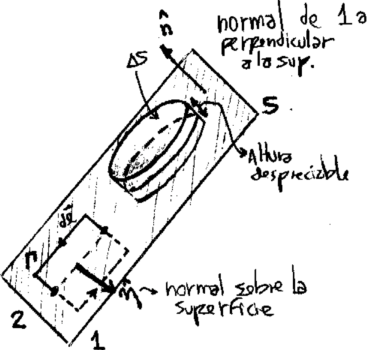
\includegraphics[width=0.4\textwidth]{images/fig_ft1_contorno1.pdf}	 
	\end{center}
	\caption{}
\end{figure} 
y puesto que vale la permutación
\[
	0 = ( -\vb{E}_2 + \vb{E}_1 )\cdot(\hat{n}\times\hat{\eta}) \longrightarrow 
	0 = \hat{\eta} \cdot ( ( -\vb{E}_2 + \vb{E}_1 ) \times \hat{n} )
\]

de modo que la componente tangencial es continua y entonces
\[
	\hat{n} \times ( \vb{E}_2 - \vb{E}_1 ) = 0
\]
\[
	E_{2\hat{n}} - E_{1\hat{n}} = 4 \pi \sigma \qquad \qquad E_{2\hat{t}} -E_{1\hat{t}} = 0
\]
\[
	-\Nabla\phi_2\cdot\hat{n} + \Nabla\phi_1\cdot\hat{n} = 4 \pi \sigma
\]
\[
	\frac{\Nabla(\phi_2-\phi_1)\cdot \hat{n}}{4 \pi} = \sigma
\]
\[
	\sigma = \frac{1}{4\pi}\dpar{(\phi_1-\phi_2)}{n}
\]
esta es la densidad de carga inducida sobre la frontera entre medios.

Para los medios magnéticos
\[
	\rotorm{H} = \frac{4 \pi}{c} \vb{J}_l
\]
\[
	\int_S (\rotorm{H}) \cdot d\vb{S} = \int_S \frac{4 \pi}{c} \vb{J}_l \cdot d\vb{S} = 
	\frac{4 \pi}{C} \vb{g}_l\cdot \hat{s} d\ell
\]
donde hicimos la transformación
\[
	\int \vb{H}\cdot d\ell = (\vb{H}_2-\vb{H}_1)\cdot d\ell
\]
y donde recordemos que la altura de $\Gamma$ tiene a cero.
\[
	\frac{4 \pi}{c} \vb{g}_l \cdot \vb{s} = ( -\vb{H}_2 + \vb{H}_1 )\cdot( \hat{n} \times \hat{s} ) d\ell
\]
\[
	\frac{4 \pi}{c} \vb{g}_l \cdot \vb{s} \; d\ell = (\vb{H}_1 -\vb{H}_2 \times \hat{n})\cdot \hat{s} 
d\ell
\]

\begin{figure}[htb]
	\begin{center}
	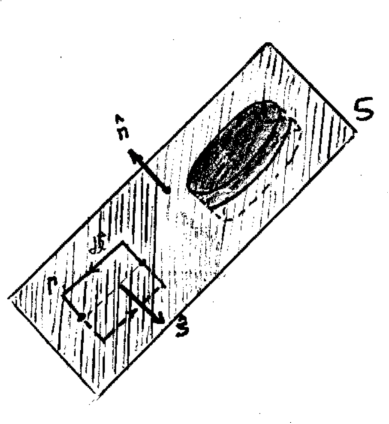
\includegraphics[width=0.4\textwidth]{images/fig_ft1_contorno2.pdf}	 
	\end{center}
	\caption{}
\end{figure} 

de manera que 
\[
	\frac{4 \pi}{c} \vb{g}_l = \hat{n} \times ( \vb{H}_2 - \vb{H}_1 )
\]
\[
	\hat{n}\times\hat{s} = \frac{d\vb{\ell}}{d\ell} 
\]
\[
	B_{2\hat{n}} - B_{1\hat{n}} = 0 \qquad \qquad H_{2\hat{t}} - H_{1\hat{t}} = \frac{4 \pi}{c} g_l
\]
\[
	\int_S \vb{B}\cdot d\vb{S} = 0 \Rightarrow (\vb{B}_2 - \vb{B}_1 )\cdot\hat{n} = 0
\]

% =================================================================================================
\section{Desarrollo multipolar}
% =================================================================================================

\[
	\phi(\vb{x}) = \int_{V'} \frac{\rho(\v{x})}{|\vb{x}-\vb{x}'|} \; dV'
\]
Cuando la expresión es muy complicada podemos desarrollarla en una serie de potencias
\[
	\phi(\vb{x}) = \frac{Q}{|\vb{x}|} + \frac{\vb{x}\cdot\vb{p}}{|\vb{x}|^3} +
	\sum_{i,j}^3 \frac{1}{2|\vb{x}|^5} x_i Q_{ij} x_j
\]
donde está centrado en el origen de coordenadas.

% \bibliographystyle{CBFT-apa-good}	% (uses file "apa-good.bst")
% \bibliography{CBFT.Referencias} % La base de datos bibliográfica

\end{document}
